\documentclass[12pt,a4paper]{article}
\usepackage[margin=2.5cm]{geometry}
\usepackage{graphicx,booktabs,array,amsmath,siunitx,natbib,caption,subcaption,placeins,setspace,lineno,url}
\usepackage[hidelinks]{hyperref}
\graphicspath{{figures/}}
\sisetup{separate-uncertainty=true,per-mode=symbol,range-phrase={--},range-units=single}
\onehalfspacing
\linenumbers

\title{Gas-specific precision and vertical concentration gradients across spatio-temporal resolutions in a naturally ventilated dairy barn}
\author{Harsh Sahu$^{a,b}$, Long Chen$^{a}$, Thomas Amon$^{a,b}$, David Janke$^{a,*}$}
\date{}

\begin{document}
\maketitle
\begin{center}\small
$^{a}$Leibniz Institute for Agricultural Engineering and Bioeconomy (ATB), Max-Eyth-Allee 100, 14469 Potsdam, Germany\\
$^{b}$Institute of Animal Hygiene and Environmental Health, Department of Veterinary Medicine, Freie Universit\"at Berlin, Germany\\
$^{*}$Corresponding author: \href{mailto:djanke@atb-potsdam.de}{djanke@atb-potsdam.de}
\end{center}

\begin{abstract}
Concentration measurements in naturally ventilated dairy barns are often interpreted as though spatial and temporal averaging affected all gases similarly. This assumption was tested by measuring carbon dioxide (\(\mathrm{CO_2}\)), methane (\(\mathrm{CH_4}\)), and ammonia (\(\mathrm{NH_3}\)) at 51 internal sampling points arranged as 17 vertical triplets during Campaign~1, followed by a 32-point top-and-bottom network during Campaign~2. Two cavity ring-down spectrometers and, in Campaign~1, two Fourier-transform infrared spectrometers sampled sequentially at four-minute resolution. Fourier-transform infrared concentrations were harmonised to the cavity ring-down scale after a 24-h co-location test. Precision was quantified as the spatial coefficient of variation at hourly, daily, weekly, and whole-period resolutions. Linear mixed-effects models tested height, period, and their interaction; gas ratios were analysed to distinguish gas-specific gradients from common dilution. Precision depended strongly on gas and temporal aggregation (response-by-scale interaction, \(p<0.001\)). Median hourly spatial coefficients of variation were approximately 7.5--8.9\% for \(\mathrm{CO_2}\), 22.0--27.2\% for \(\mathrm{CH_4}\), and 24.3--33.2\% for \(\mathrm{NH_3}\), and generally decreased at daily and weekly scales. Height effects and height-by-period interactions were significant for all concentrations and ratios (\(p<0.001\)). Top concentrations exceeded bottom concentrations most consistently in autumn; in summer, the vertical increase was weaker and not universal across horizontal positions. Thus, the hypothesis of gas-specific spatio-temporal precision was supported, whereas the hypothesised general increase with sampling height was seasonally conditional. The middle height, \SI{3.6}{m} above the floor and only \SI{1}{m} above the bottom points, added comparatively little vertical separation during summer, supporting its omission as a practical consequence of the heterogeneity analysis rather than as evidence of homogeneous mixing.
\end{abstract}

\noindent\textbf{Keywords:} ammonia; dairy housing; methane; mixing ratio; sampling height; spatial coefficient of variation

\section*{Nomenclature}
\begin{tabular}{>{\raggedright\arraybackslash}p{2.2cm}>{\raggedright\arraybackslash}p{10.8cm}}
\toprule Symbol & Definition\\ \midrule
CRDS & cavity ring-down spectroscopy\\
CV & coefficient of variation, \%\\
FTIR & Fourier-transform infrared spectroscopy\\
NVDB & naturally ventilated dairy barn\\
RE & relative error against the contemporaneous dense-network mean, \%\\
SD & standard deviation\\
SP & sampling point\\ \bottomrule
\end{tabular}

\section{Introduction}
Emission estimates for naturally ventilated livestock buildings depend jointly on airflow and the concentration field sampled across that airflow. Wind, buoyancy, animals, manure surfaces and internal obstructions produce spatially variable transport, so analytical accuracy alone does not ensure spatial representativeness \citep{Calvet2013,Ogink2013}. Direct wind-tunnel measurements demonstrated that combining concentration and velocity at one constant height could produce emission errors up to 97\%, whereas vertically resolved sampling reduced the error to below 5\% in the tested cases \citep{Janke2020}. A concentration sensor should therefore be evaluated at the spatial and temporal resolution at which it will be used.

Vertical gradients are gas- and site-specific. \citet{Sahu2023} measured significant height effects for \(\mathrm{CO_2}\), \(\mathrm{CH_4}\), and \(\mathrm{NH_3}\) at the outlet of a naturally ventilated dairy building and commonly observed greater concentrations near the top. In another open dairy barn, \(\mathrm{NH_3}\) was greatest near the floor whereas \(\mathrm{CH_4}\) was greatest at the upper level, demonstrating that a universal vertical ordering cannot be assumed \citep{Durso2024}. Horizontal sampling density also affects inferred means and variability \citep{Durso2022,DeVogeleer2017}. \citet{Doumbia2021} further showed that the frequently used approximately \SI{3}{m} sampling height represented well-mixed conditions only for a subset of simulated convection cases. These results motivate measurements both near the customary height and at uncommon vertical extremes.

Temporal aggregation is equally important. Rapid changes in wind and thermal forcing may create large short-term spatial differences that are attenuated in daily or campaign means. Wind direction can also change which openings are inlets or outlets and which indoor locations are representative \citep{Saha2013,Koenig2018,JankeSampling2020}. Regional meteorological observations describe the synoptic forcing but do not replace velocity measurements at the barn openings. Consequently, seasonal comparisons should quantify temporal evolution while avoiding causal claims that cannot be resolved without co-located airflow measurements.

Gas ratios provide a complementary diagnostic. If all gases respond identically to dilution, their ratios should be spatially more stable than their concentrations. Persistent gradients in \(\mathrm{NH_3}/\mathrm{CO_2}\), \(\mathrm{CH_4}/\mathrm{CO_2}\), or \(\mathrm{NH_3}/\mathrm{CH_4}\) instead indicate differences in sources, sinks or transport. Information-based measures can additionally identify redundant locations, although the entropy optimisation of \citet{Chen2026} was developed for CFD-derived ventilation fields and must be interpreted here as an empirical adaptation rather than a direct replication.

Two hypotheses were tested: (H1) the precision of each gas differs at different spatial and temporal resolutions; and (H2) gas concentrations generally increase with increasing vertical sampling height, as suggested by previous measurements \citep{Sahu2023}. The objectives were to quantify concentration and ratio heterogeneity from hourly to campaign scales, determine whether the vertical pattern persisted from summer through winter, and evaluate omission of the middle layer as a practical consequence of the observed structure.

\section{Materials and methods}
\subsection{Barn and sampling layout}
Measurements were conducted in an occupied NVDB at Gross Kreutz, Brandenburg, Germany. The barn was \SI{38.88}{m} long and \SI{17.65}{m} wide, with an internal airspace of approximately \SI{4529}{m^3} and capacity for 58 dairy cows. Seventeen horizontal positions covered lying, feeding, walking and manure-adjacent zones (Fig.~\ref{fig:layout}). At every position, a vertical triplet comprised a top SP \SI{0.60}{m} below the local roof, a middle SP \SI{3.60}{m} above the floor, and a bottom SP \SI{2.60}{m} above the floor. Thus, the middle and bottom layers were separated by only \SI{1.00}{m}; the top layer followed the sloping roof and represented an intentionally uncommon near-roof position.

\begin{figure}[htbp]
\centering
\begin{subfigure}[t]{0.99\textwidth}\centering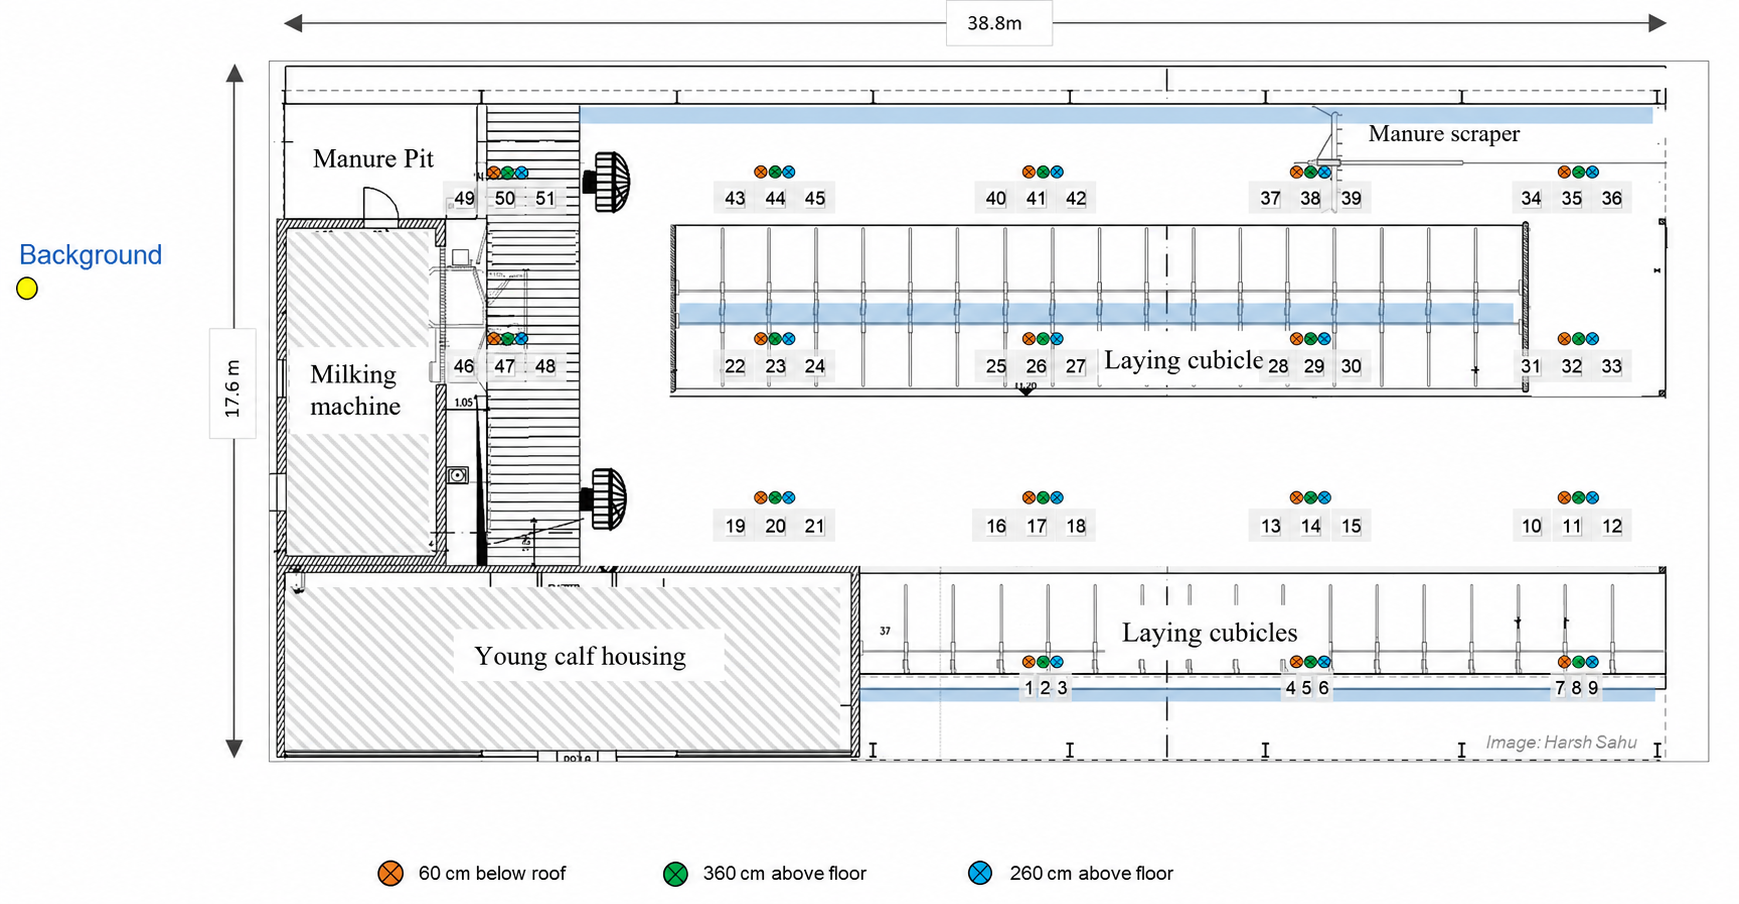
\includegraphics[width=\linewidth]{Fig1a_campaign1_sampling_layout_no_ringline.png}\caption{Plan view and 51 internal SPs.}\end{subfigure}
\begin{subfigure}[t]{0.83\textwidth}\centering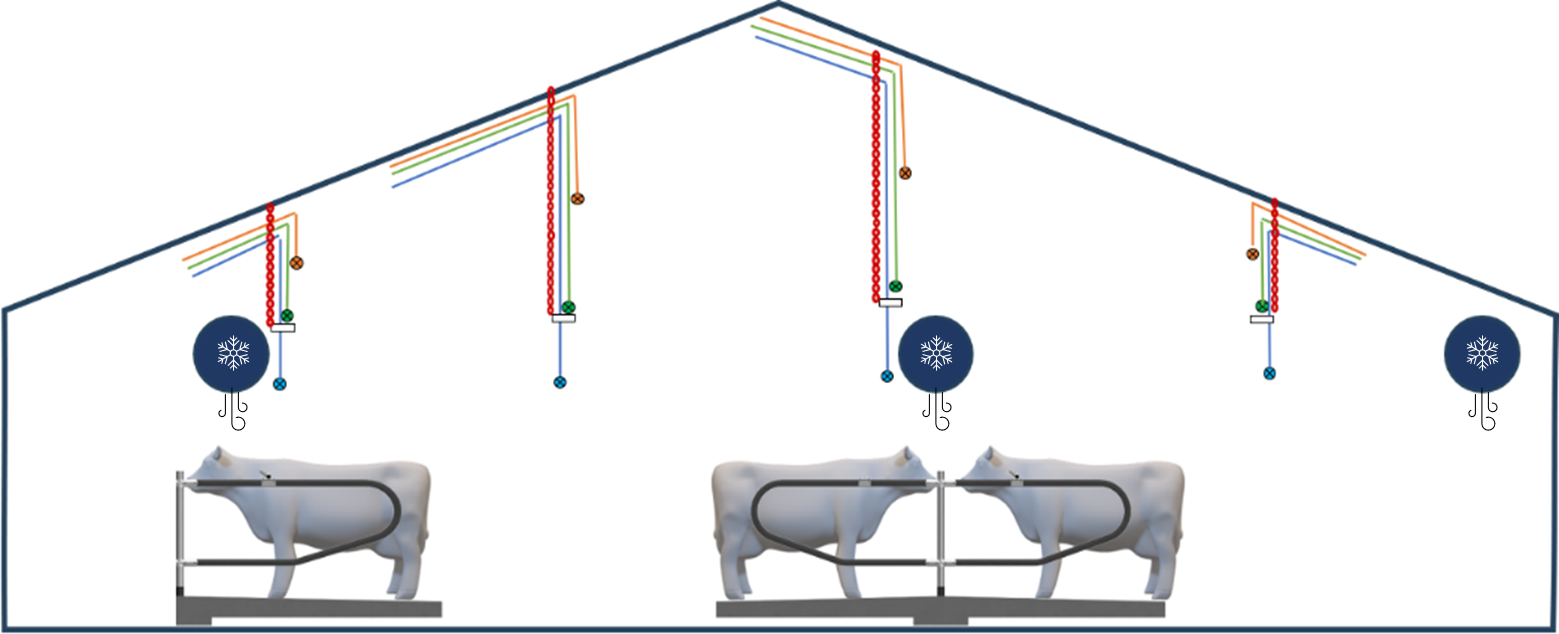
\includegraphics[width=\linewidth]{Fig1b_barn_cross_section.png}\caption{Vertical arrangement of the sampling tubes.}\end{subfigure}
\caption{Experimental barn and sampling design. Location numbers increase in vertical triplets: top, middle and bottom. The plan also shows functional zones and mechanical mixing fans.}
\label{fig:layout}
\end{figure}

\subsection{Campaigns and gas measurements}
Campaign~1 combined dense observations from June--August 2024 (summer; 90 measurement dates) and 1--24 October 2024 (autumn; 24 dates). All 51 internal SPs were measured with two CRDS and two FTIR analysers. Campaign~2 used the reduced top-and-bottom design, measured by two CRDS analysers from 16 November to 31 December 2024 (15 late-autumn and 31 winter dates). Thirty-two positions were operational because two previously identified positions were omitted for pragmatic reasons. Sampling proceeded sequentially at four-minute resolution. The first \SI{60}{s} after switching was discarded and the remaining \SI{180}{s} were averaged; the time stamp represented the end of the averaging interval.

A preliminary 24-h co-located field comparison was performed before Campaign~1. Two polytetrafluoroethylene sampling lines terminated at the same central barn position; one line was divided between the CRDS instruments and the other between the FTIR instruments. FTIR values were 6\% higher for \(\mathrm{CO_2}\) and \(\mathrm{CH_4}\), and 9\% higher for \(\mathrm{NH_3}\). Campaign~1 FTIR values were therefore harmonised as \(C_{\mathrm{CO_2,corr}}=C_{\mathrm{CO_2,raw}}/1.06\), \(C_{\mathrm{CH_4,corr}}=C_{\mathrm{CH_4,raw}}/1.06\), and \(C_{\mathrm{NH_3,corr}}=C_{\mathrm{NH_3,raw}}/1.09\). CRDS values were unchanged. Only missing, zero or negative gas values were excluded; all positive concentrations were retained.

\subsection{Meteorological context}
Hourly temperature, relative humidity, precipitation, wind speed and wind direction were obtained from the German Meteorological Service for the nearest suitable station and aligned in UTC \citep{DWD2024}. Wind roses and temperature--humidity time series were used to describe seasonal forcing. Westerly flow was defined as 225--315\(^{\circ}\). Hourly internal concentration means under westerly and other directions were compared using Wilcoxon tests, and exploratory mixed models included wind speed, direction class, temperature, relative humidity and precipitation. These analyses describe association, not barn-scale causation, because velocity and direction were not measured simultaneously at every opening.

\subsection{Responses and statistical analysis}
Ratios were calculated on paired observations as
\begin{equation}
R_{a/b}=100\,C_a/C_b .
\end{equation}
Spatial precision within each hour, day, ISO week and campaign period was expressed as
\begin{equation}
\mathrm{CV}_{g,t}=100\,\frac{\mathrm{SD}_{i}(C_{g,i,t})}{\overline{C}_{g,t}},
\end{equation}
where \(i\) is SP and \(t\) is aggregation interval. Because ratio distributions can be sensitive to small denominators, medians and interquartile ranges of block-level CVs were emphasised alongside campaign means and SDs. A mixed model tested log-transformed CV with response, temporal scale and their interaction as fixed effects and period as a random intercept.

For dense Campaign~1 observations, log response was modelled with height, period and their interaction as fixed effects and horizontal position and date as crossed random intercepts. A second model used only locations shared by both campaigns and tested top versus bottom across four periods, again with horizontal position and date as random effects. Tukey-adjusted estimated-marginal-mean contrasts were calculated. The consistency of H2 was further expressed as the number of horizontal positions at which \(\overline C_{\rm top}>\overline C_{\rm middle}>\overline C_{\rm bottom}\).

For complete two-hour dense-network blocks, each single-height mean was compared with the 51-location mean:
\begin{equation}
\mathrm{RE}_{h,b}=100\,\frac{\overline C_{h,b}-\overline C_{{\rm dense},b}}{\overline C_{{\rm dense},b}}.
\end{equation}
Shannon entropy was calculated after discretising each response into four equiprobable bins within period. The resulting tiles assess empirical compositional information at a location; they are not estimates of airflow or local mean age of air. Analyses were conducted in R 4.5.3. Significance was assessed at \(\alpha=0.05\), with effect sizes and temporal consistency interpreted alongside \(p\)-values.

\section{Results}
\subsection{Gas-specific precision across temporal resolutions}
The analysis included 159,866 internal records: 108,078 in summer Campaign~1, 31,156 in autumn Campaign~1, 8,906 in late-autumn Campaign~2 and 11,726 in winter Campaign~2. Precision differed by response, temporal scale and their interaction (all \(p<0.001\)). At hourly resolution, median spatial CV was 7.5--8.9\% for \(\mathrm{CO_2}\), 22.0--27.2\% for \(\mathrm{CH_4}\), and 24.3--33.2\% for \(\mathrm{NH_3}\). Daily medians decreased to 4.4--6.1\%, 9.5--17.1\%, and 19.9--29.3\%, respectively. Weekly values were similar to or below daily values for \(\mathrm{CO_2}\) and \(\mathrm{CH_4}\), whereas \(\mathrm{NH_3}\) remained comparatively heterogeneous. H1 was therefore supported: both gas identity and aggregation scale altered apparent precision.

Mean concentrations also changed over time. Across heights, \(\mathrm{CO_2}\) and \(\mathrm{CH_4}\) were generally higher in autumn and winter than in summer, while \(\mathrm{NH_3}\) declined from approximately \SI{2.1}{ppm} in summer to below \SI{1}{ppm} in Campaign~2. The ratios did not track concentration changes identically, confirming that temporal variation was not a uniform multiplication of all gases.

\begin{figure}[htbp]\centering
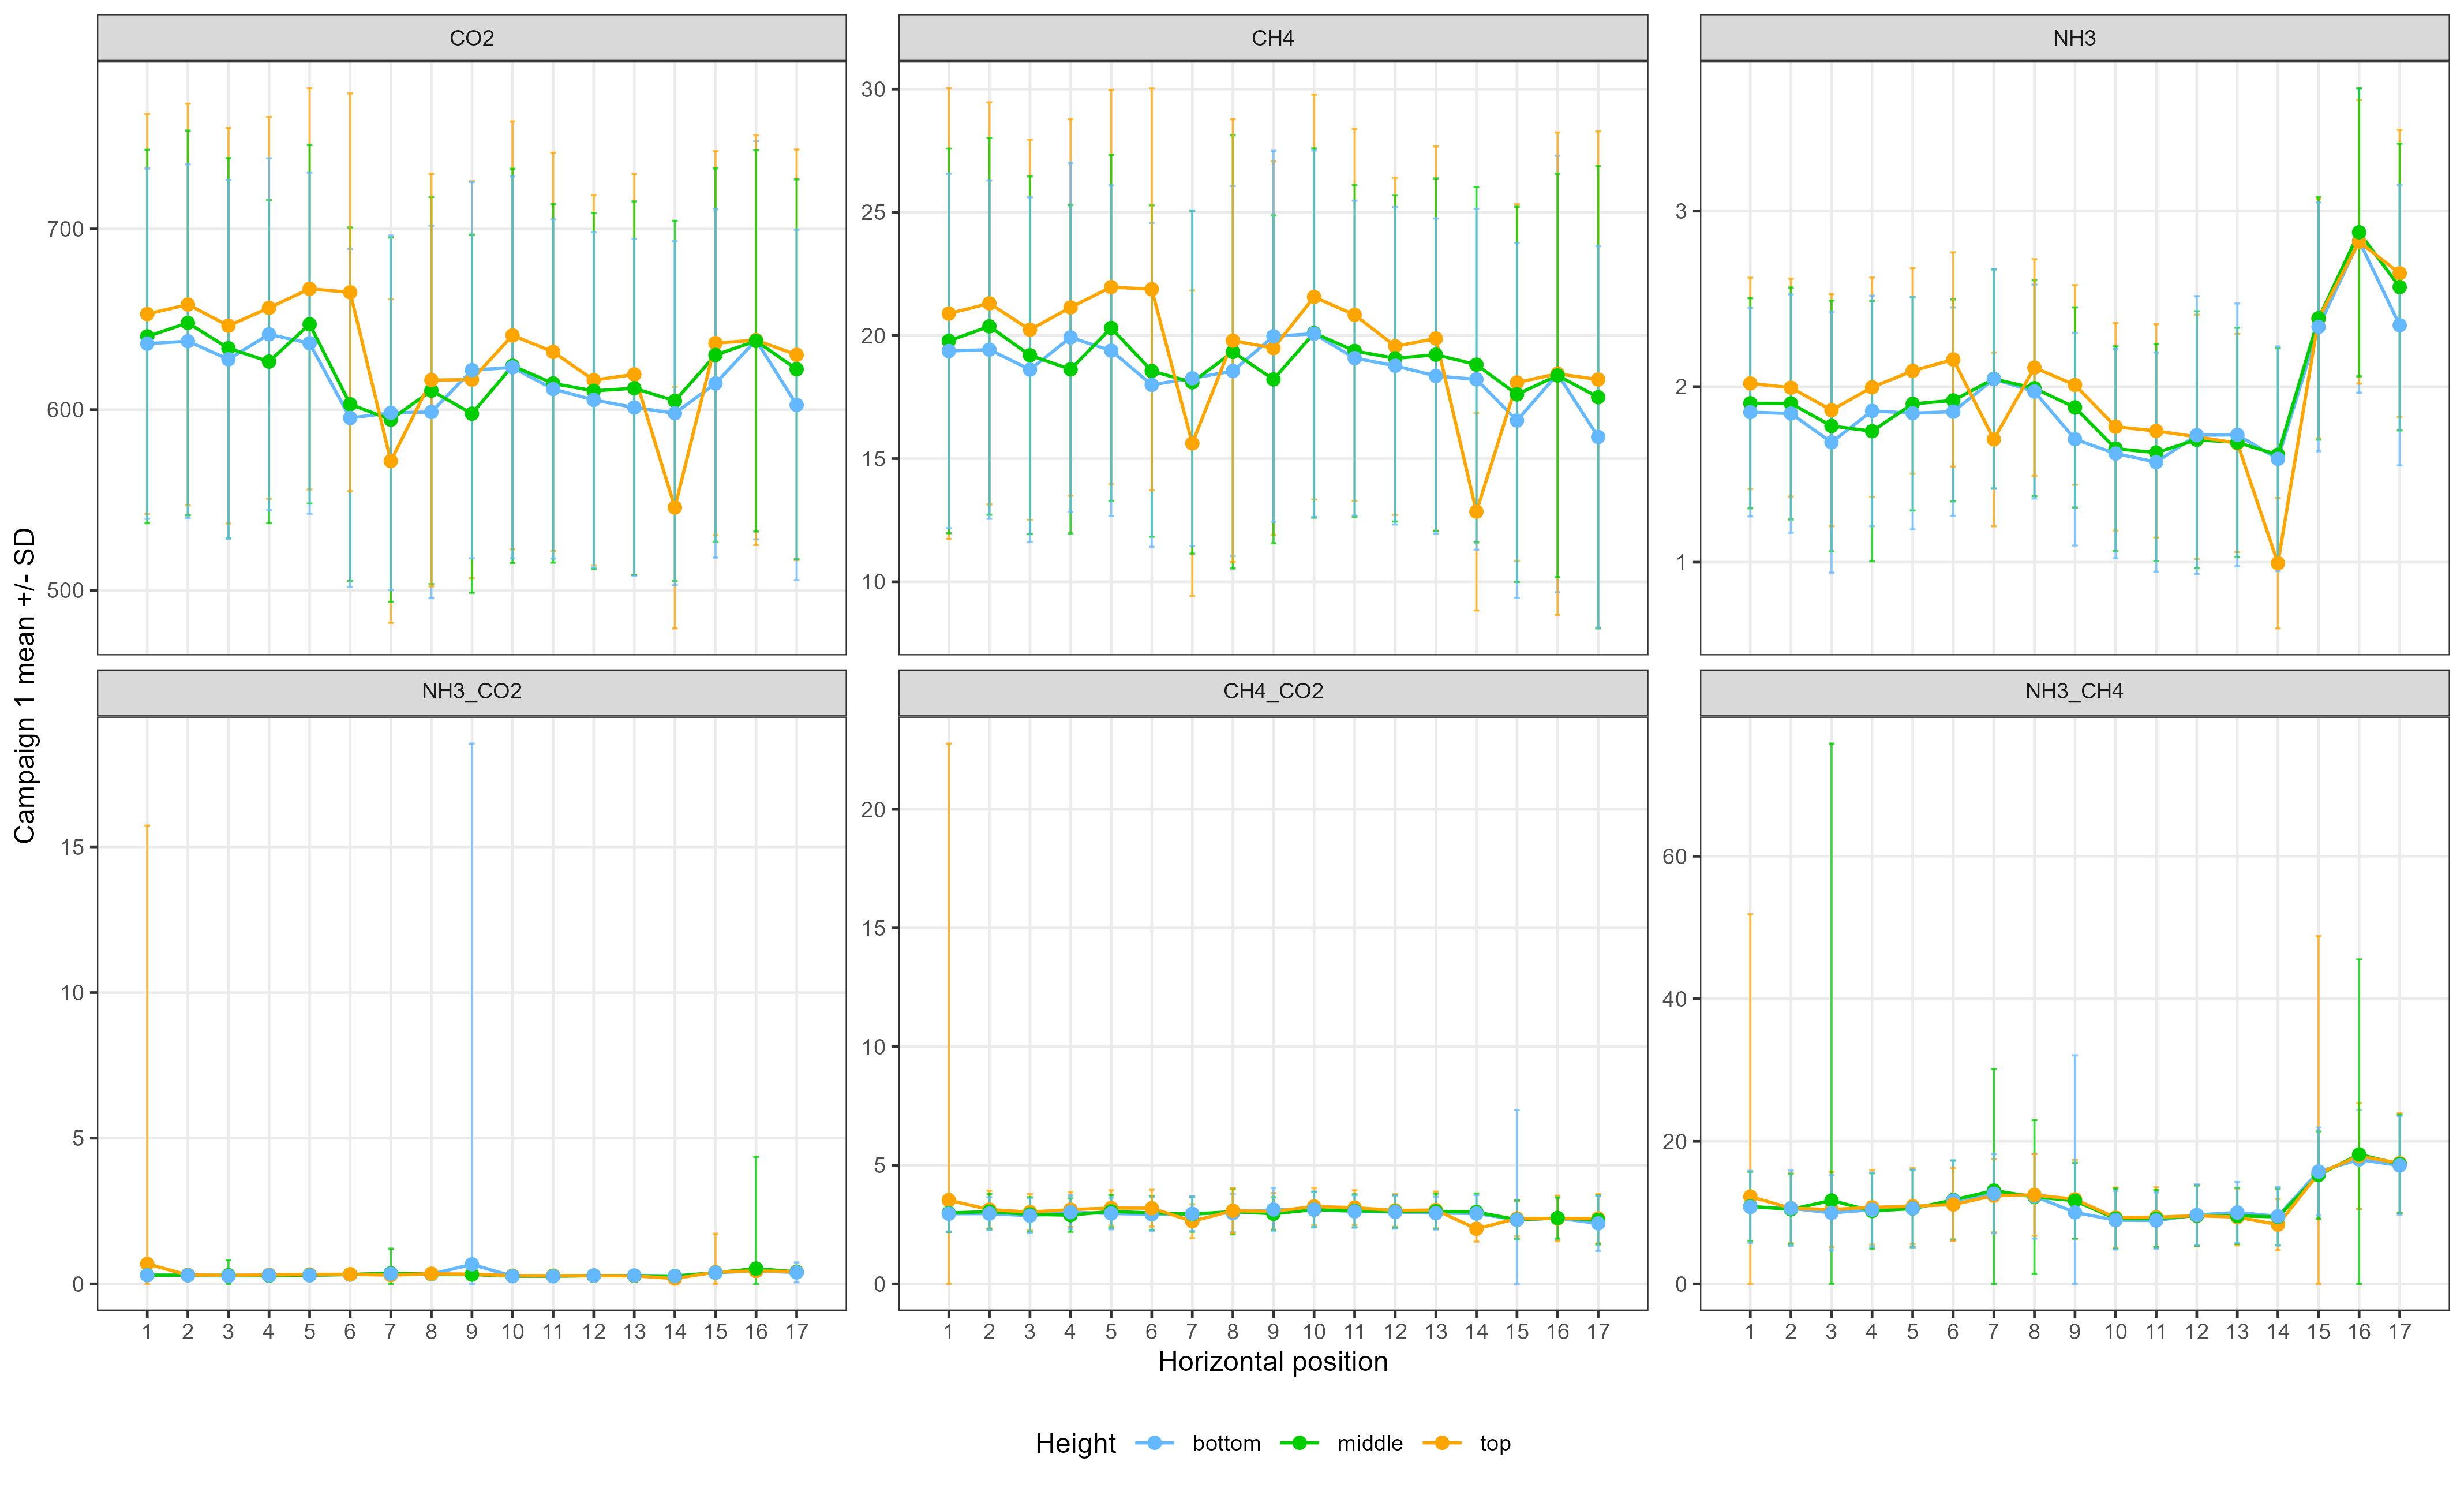
\includegraphics[width=\textwidth]{Fig2_v11_internal_means_SD.png}
\caption{Campaign~1 mean concentrations and ratios at the 17 horizontal positions, shown as mean \(\pm\) SD. The first row contains \(\mathrm{CO_2}\), \(\mathrm{CH_4}\), and \(\mathrm{NH_3}\); the second contains \(\mathrm{NH_3}/\mathrm{CO_2}\), \(\mathrm{CH_4}/\mathrm{CO_2}\), and \(\mathrm{NH_3}/\mathrm{CH_4}\). Colours denote top (orange), middle (green), and bottom (blue).}
\label{fig:means}
\end{figure}

\begin{figure}[htbp]\centering
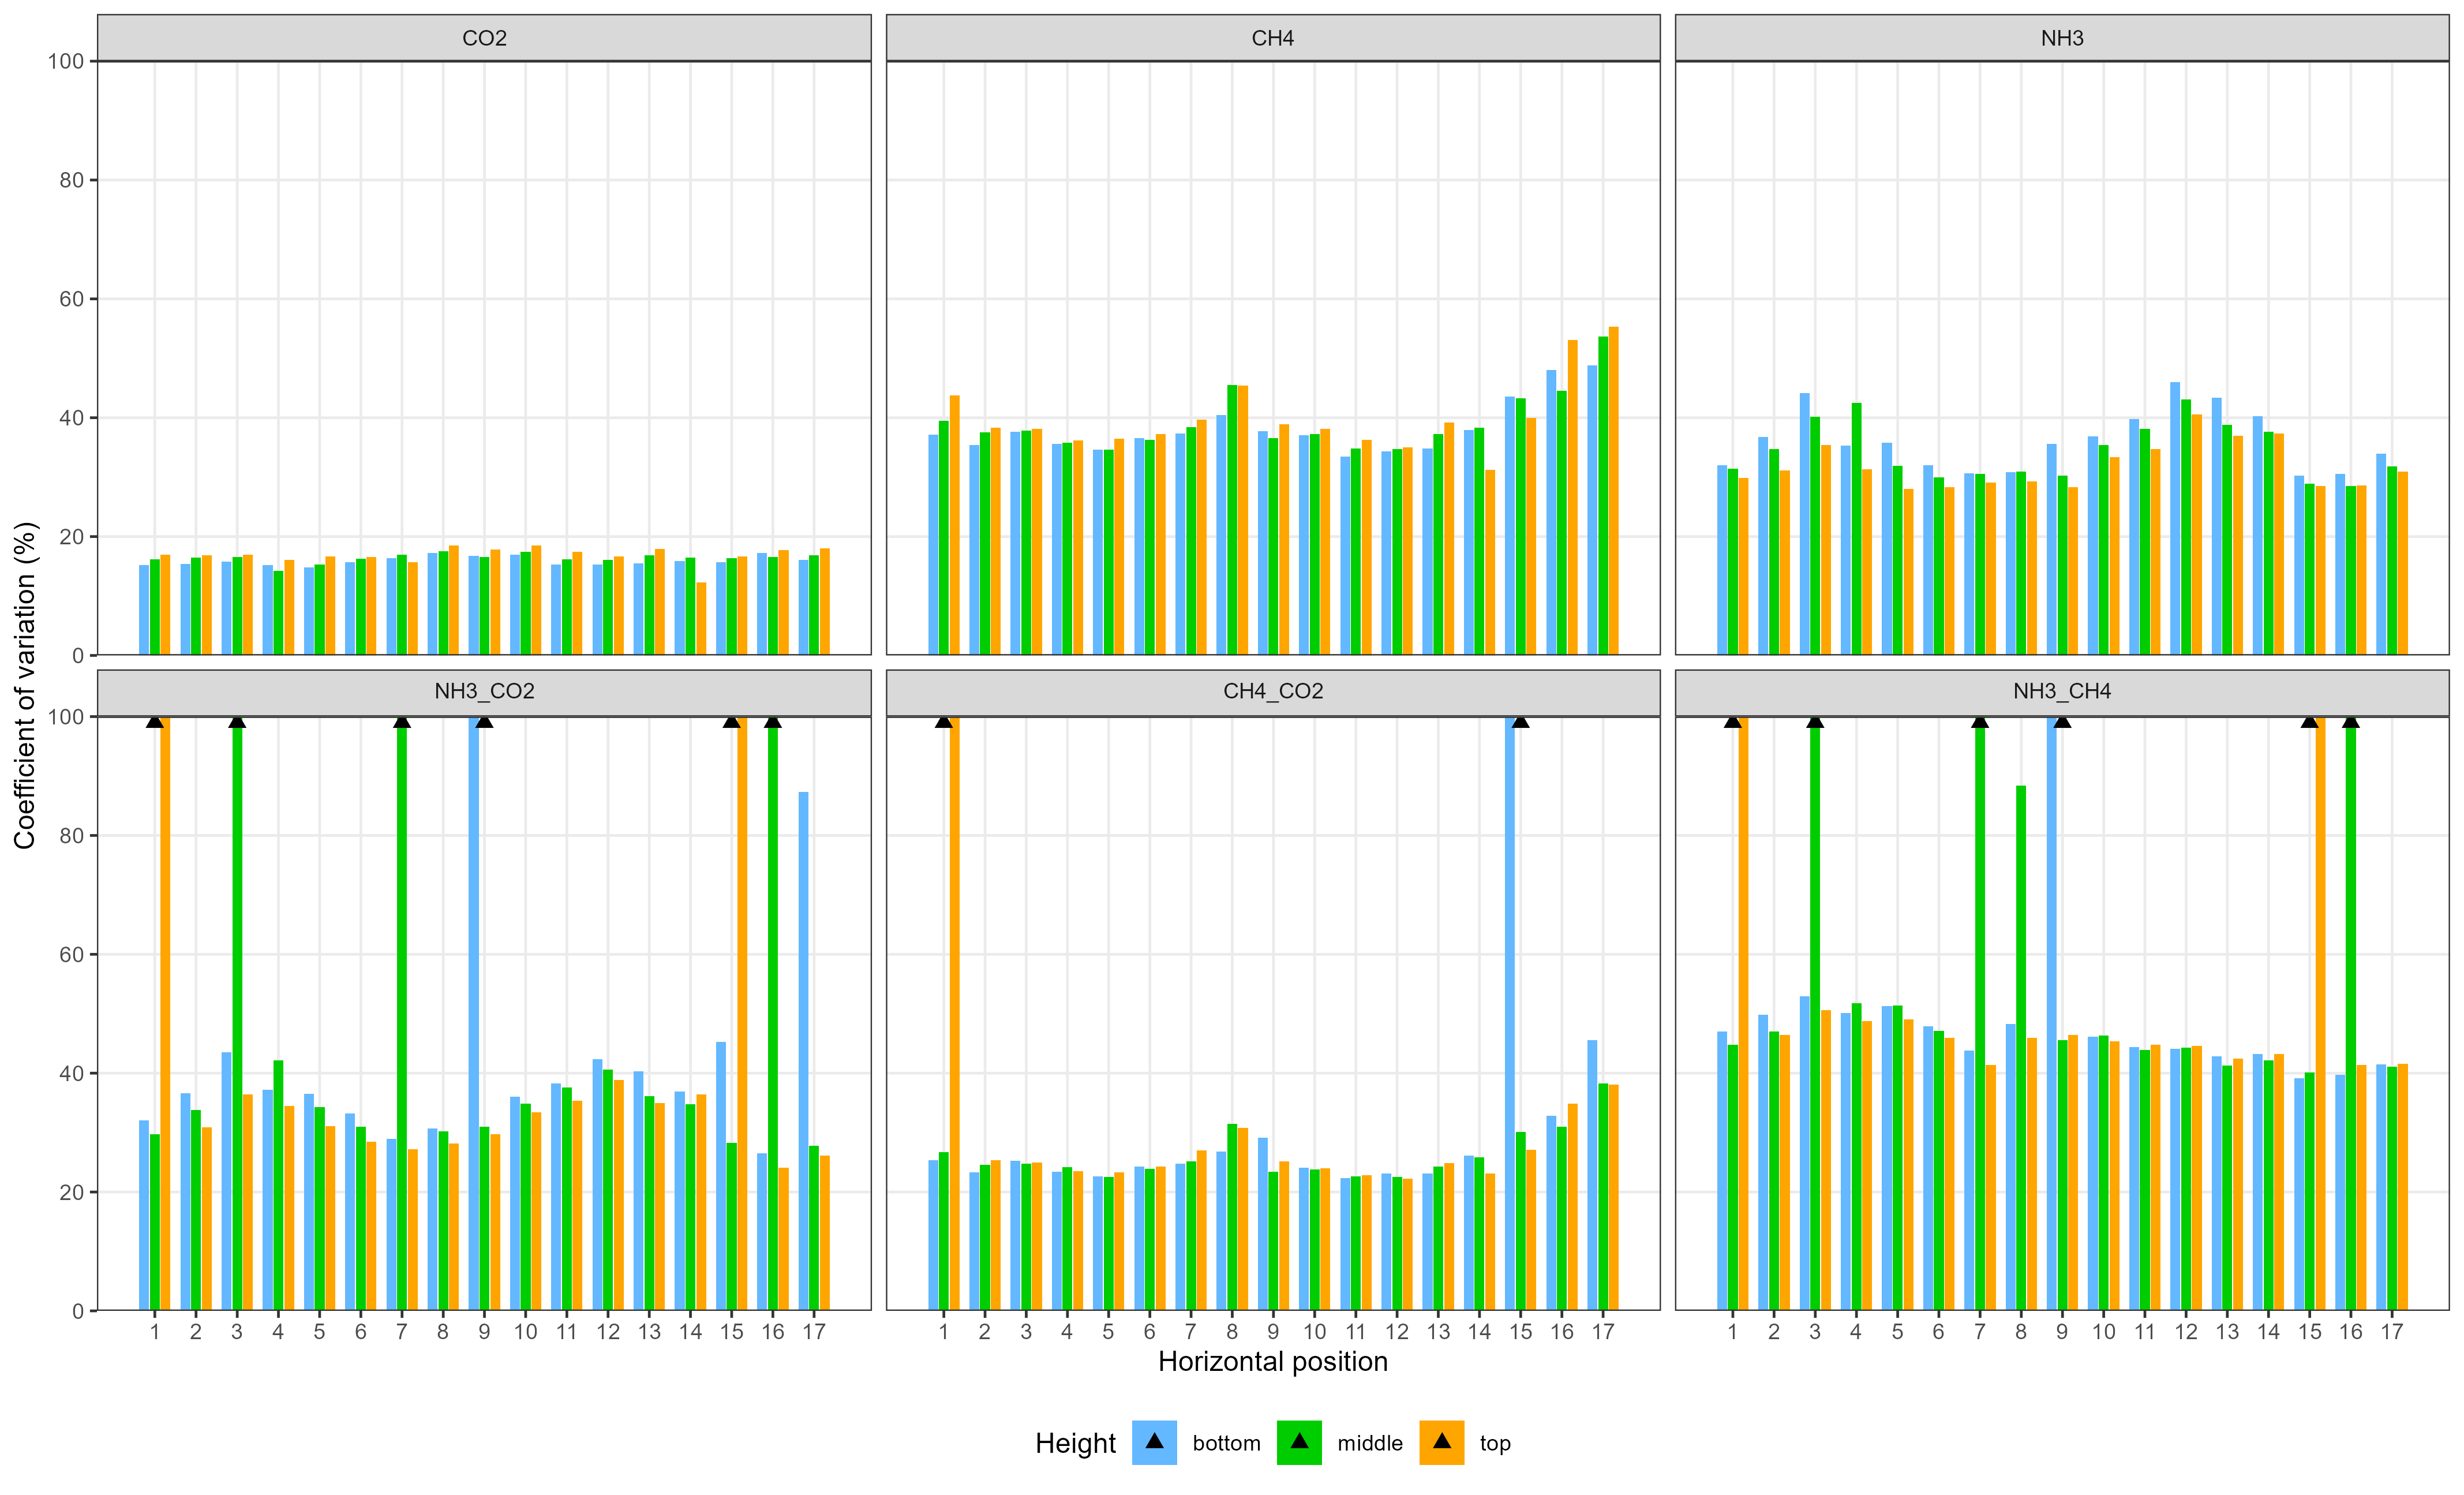
\includegraphics[width=\textwidth]{Fig2b_v11_internal_CV.png}
\caption{Spatial CV by gas, ratio and Campaign~1 period. The axis is restricted to 0--100\%; triangles at the upper boundary indicate values exceeding that display range. Separating CV from Fig.~\ref{fig:means} prevents variability from obscuring the concentration gradients.}
\label{fig:cv}
\end{figure}

\subsection{Vertical structure and its seasonal dependence}
In dense Campaign~1 data, height, period and their interaction affected every concentration and ratio (all interaction \(p<0.001\)). Summer gradients were small: geometric top means exceeded bottom means by approximately 0.9\% for \(\mathrm{CO_2}\), 1.1\% for \(\mathrm{CH_4}\), and 1.6\% for \(\mathrm{NH_3}\). In autumn, corresponding contrasts increased to approximately 4.7\%, 10.8\%, and 15.9\%. The strict top--middle--bottom ordering occurred at only 9/17, 10/17, and 10/17 positions for the three gases in summer, but at 13/17, 13/17, and 14/17 in autumn. H2 was therefore conditionally, not universally, supported.

The four-period top--bottom models confirmed significant height-by-period interactions for all responses (\(p<0.001\)). Top concentrations exceeded bottom concentrations significantly in every period except \(\mathrm{CO_2}\) in late autumn. The largest proportional separation occurred for \(\mathrm{NH_3}\), especially in autumn and winter. Ratio gradients were also significant, showing that common ventilation-driven dilution alone could not explain the vertical ordering.

\begin{figure}[htbp]\centering
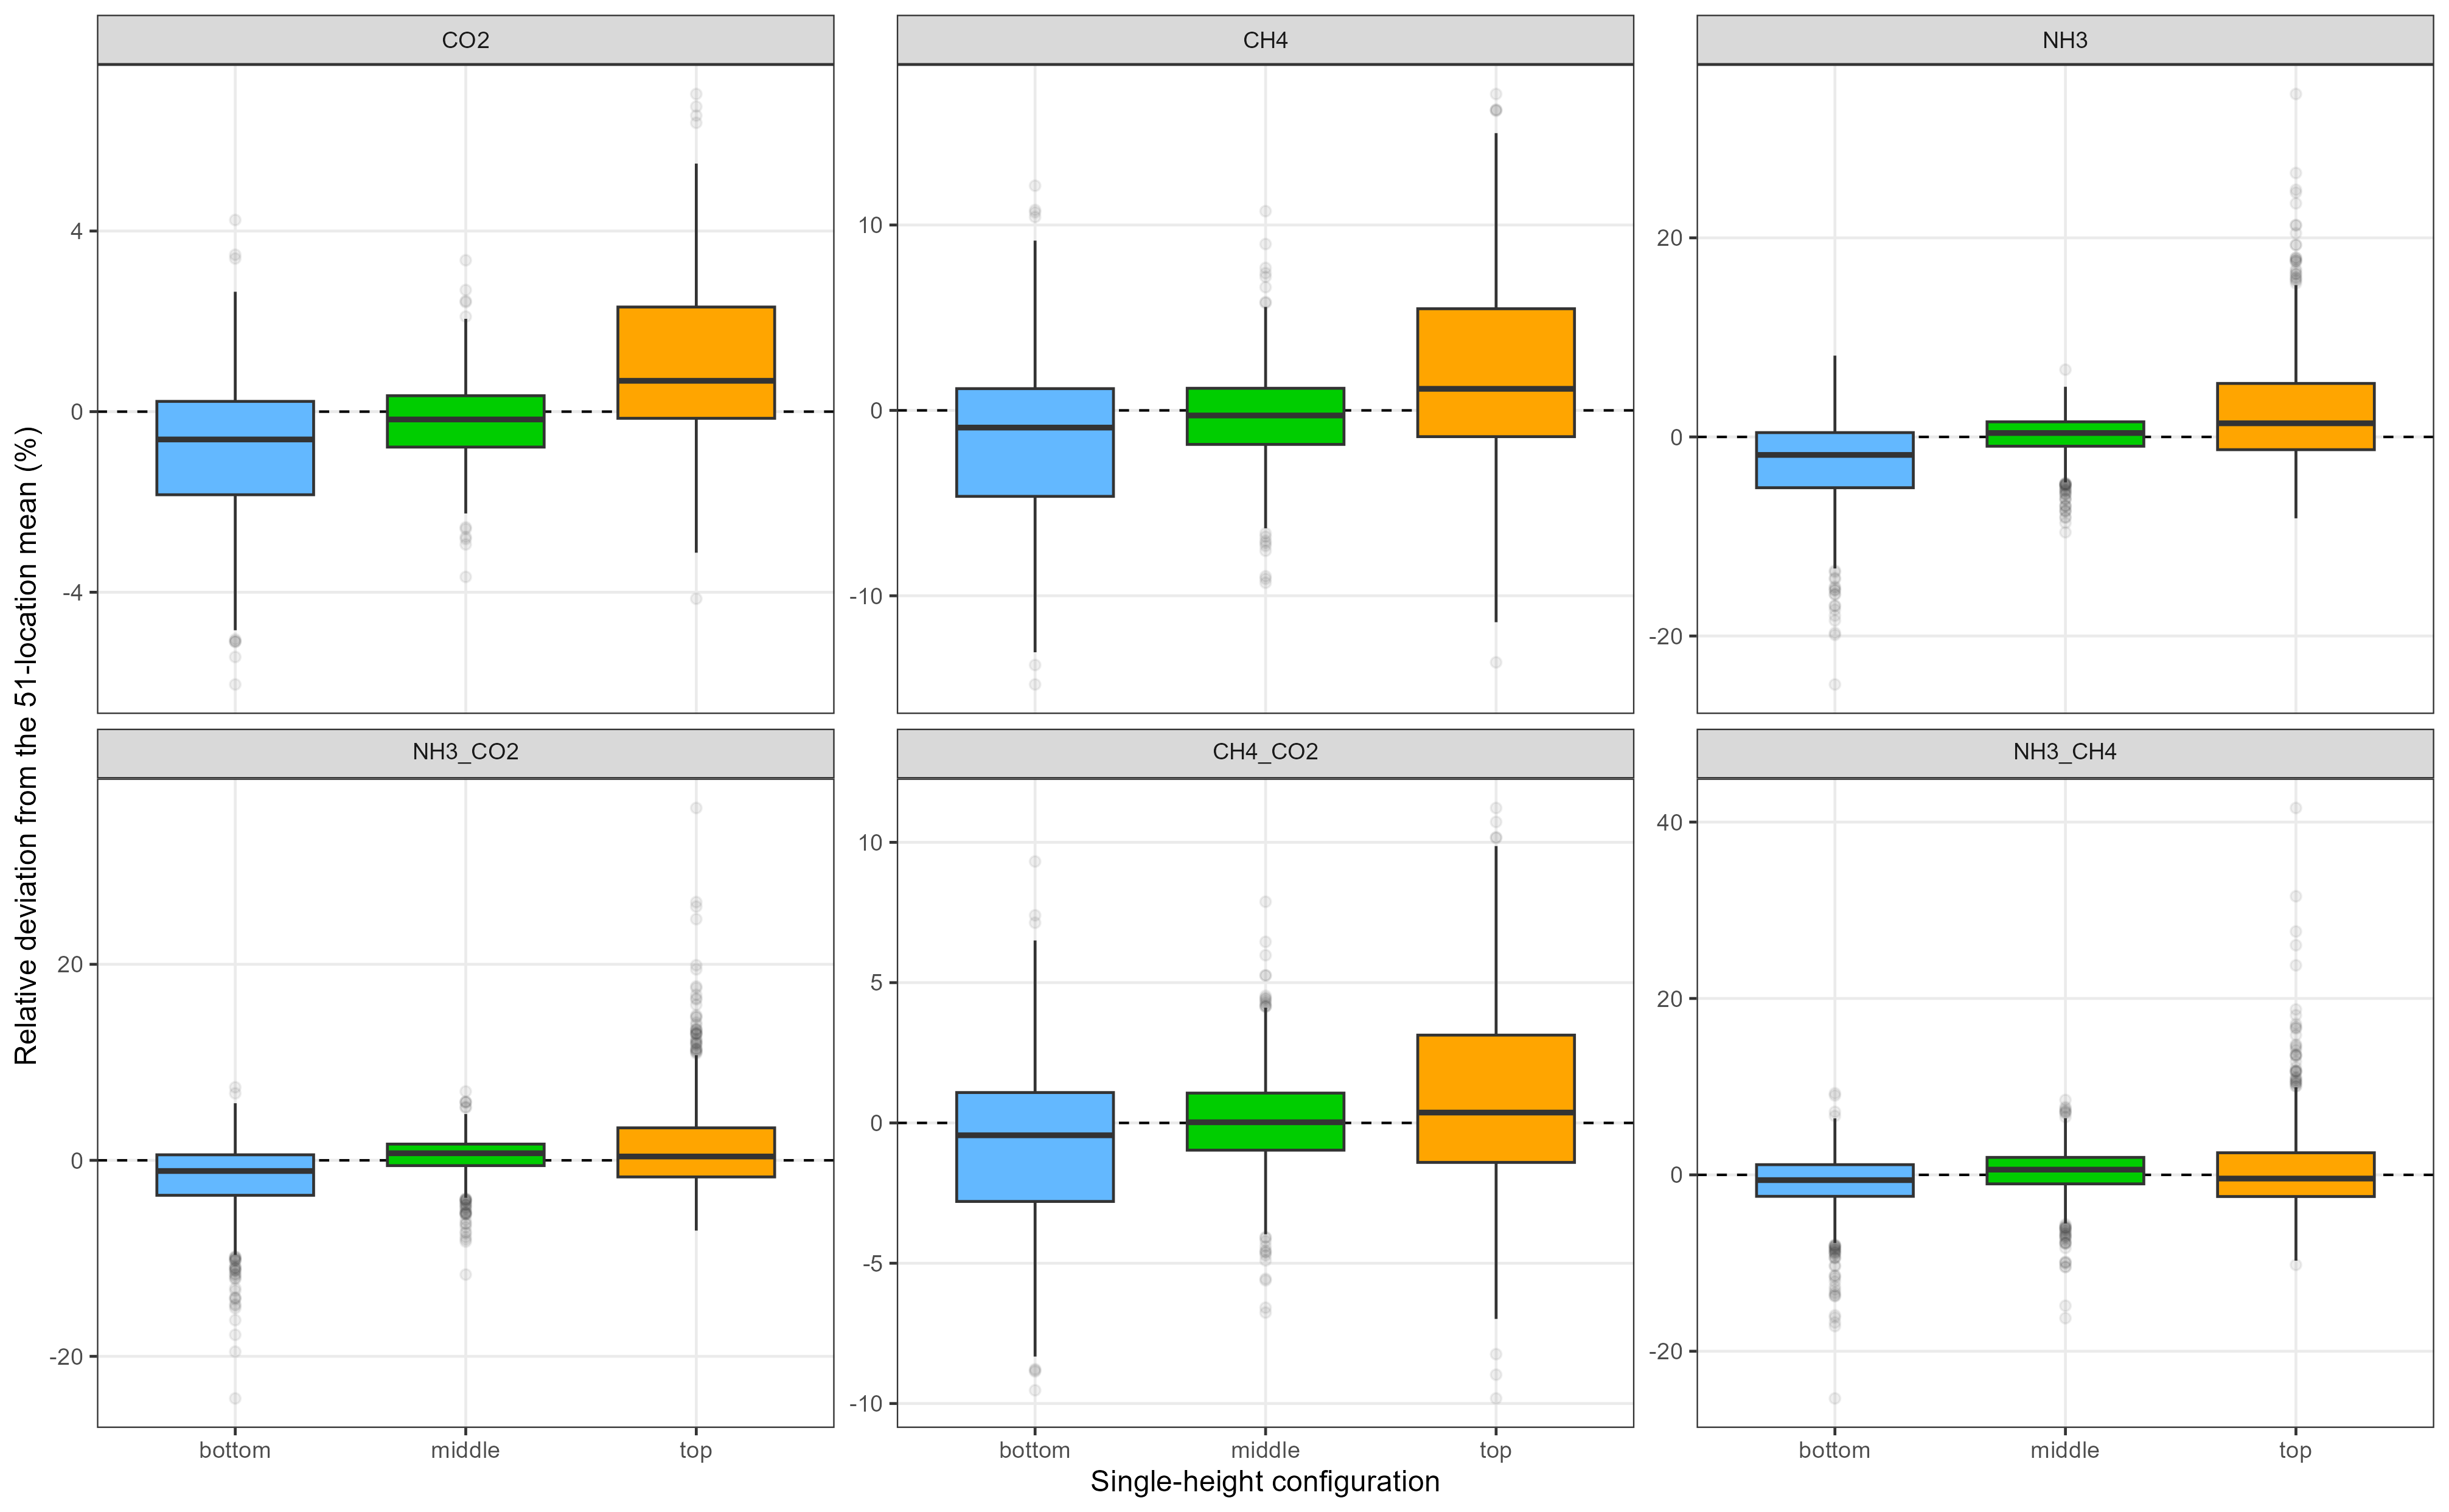
\includegraphics[width=0.92\textwidth]{Fig3_v11_single_height_relative_error.png}
\caption{Relative error of top-, middle-, and bottom-only means against the contemporaneous 51-location dense mean in 921 complete Campaign~1 two-hour blocks. Combined height configurations are intentionally omitted so that the consequences of selecting a single sampling height remain visible.}
\label{fig:re}
\end{figure}

The middle-only distribution generally lay closer to the dense mean than either extreme, as expected for an intermediate layer. Its practical incremental value was nevertheless limited during summer because it was only \SI{1}{m} above the bottom layer and frequently indistinguishable from either bottom or top for particular gases. This empirical redundancy motivated its omission in Campaign~2; it does not imply that the barn was homogeneously mixed.

\subsection{Entropy and meteorological context}
Entropy varied by gas and position (Fig.~\ref{fig:entropy}). Locations with high entropy for one gas were not invariably high for another, consistent with gas-specific source and transport behaviour. The result did not identify a universal sensor position and should not be equated with CFD-based optimisation.

\begin{figure}[htbp]\centering
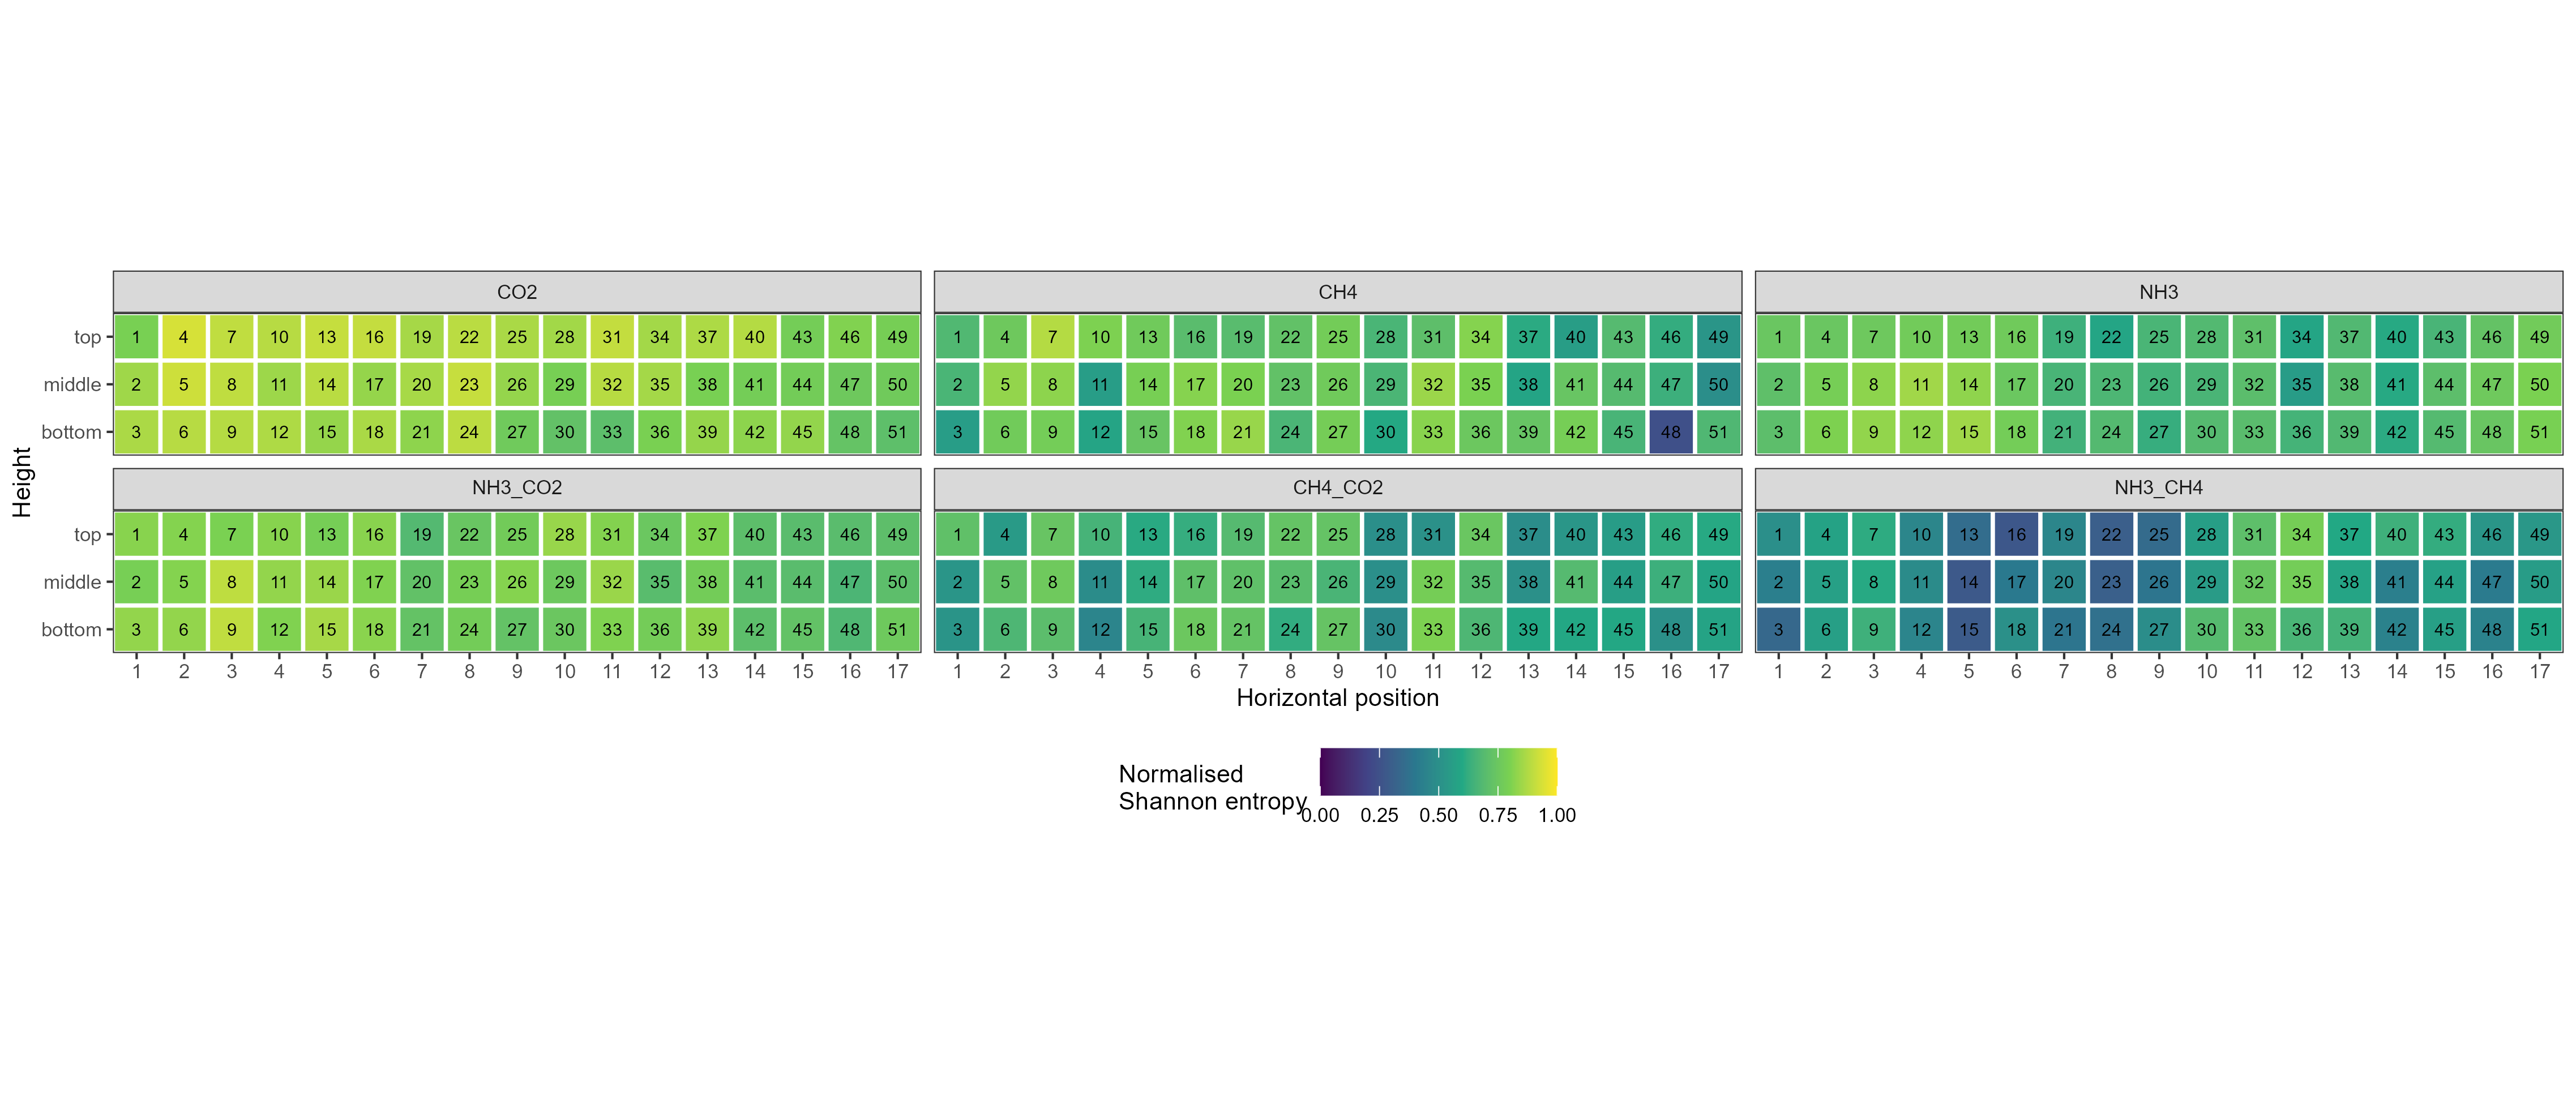
\includegraphics[width=\textwidth]{Fig4_v11_Shannon_entropy_square_tiles.png}
\caption{Four-bin Shannon entropy for each gas and ratio at horizontal positions 1--17 and the three heights during Campaign~1. Equal coordinate scaling produces square tiles. Higher entropy denotes a more even occupancy of the four concentration bins, not lower measurement uncertainty.}
\label{fig:entropy}
\end{figure}

Seasonal wind roses and temperature--humidity records showed that the campaigns sampled different external regimes (Fig.~\ref{fig:weather}). Westerly hours were associated with lower, rather than higher, internal hourly mean concentrations in the unadjusted summaries: for example, autumn Campaign~1 means changed from 671 to \SI{601}{ppm} \(\mathrm{CO_2}\), 21.3 to \SI{17.2}{ppm} \(\mathrm{CH_4}\), and 1.76 to \SI{1.37}{ppm} \(\mathrm{NH_3}\). Winter differences were also negative. These associations are consistent with enhanced ventilation under some westerly regimes, but regional wind cannot distinguish dilution from plume transport or opening-specific flow.

\begin{figure}[htbp]\centering
\begin{subfigure}[t]{0.98\textwidth}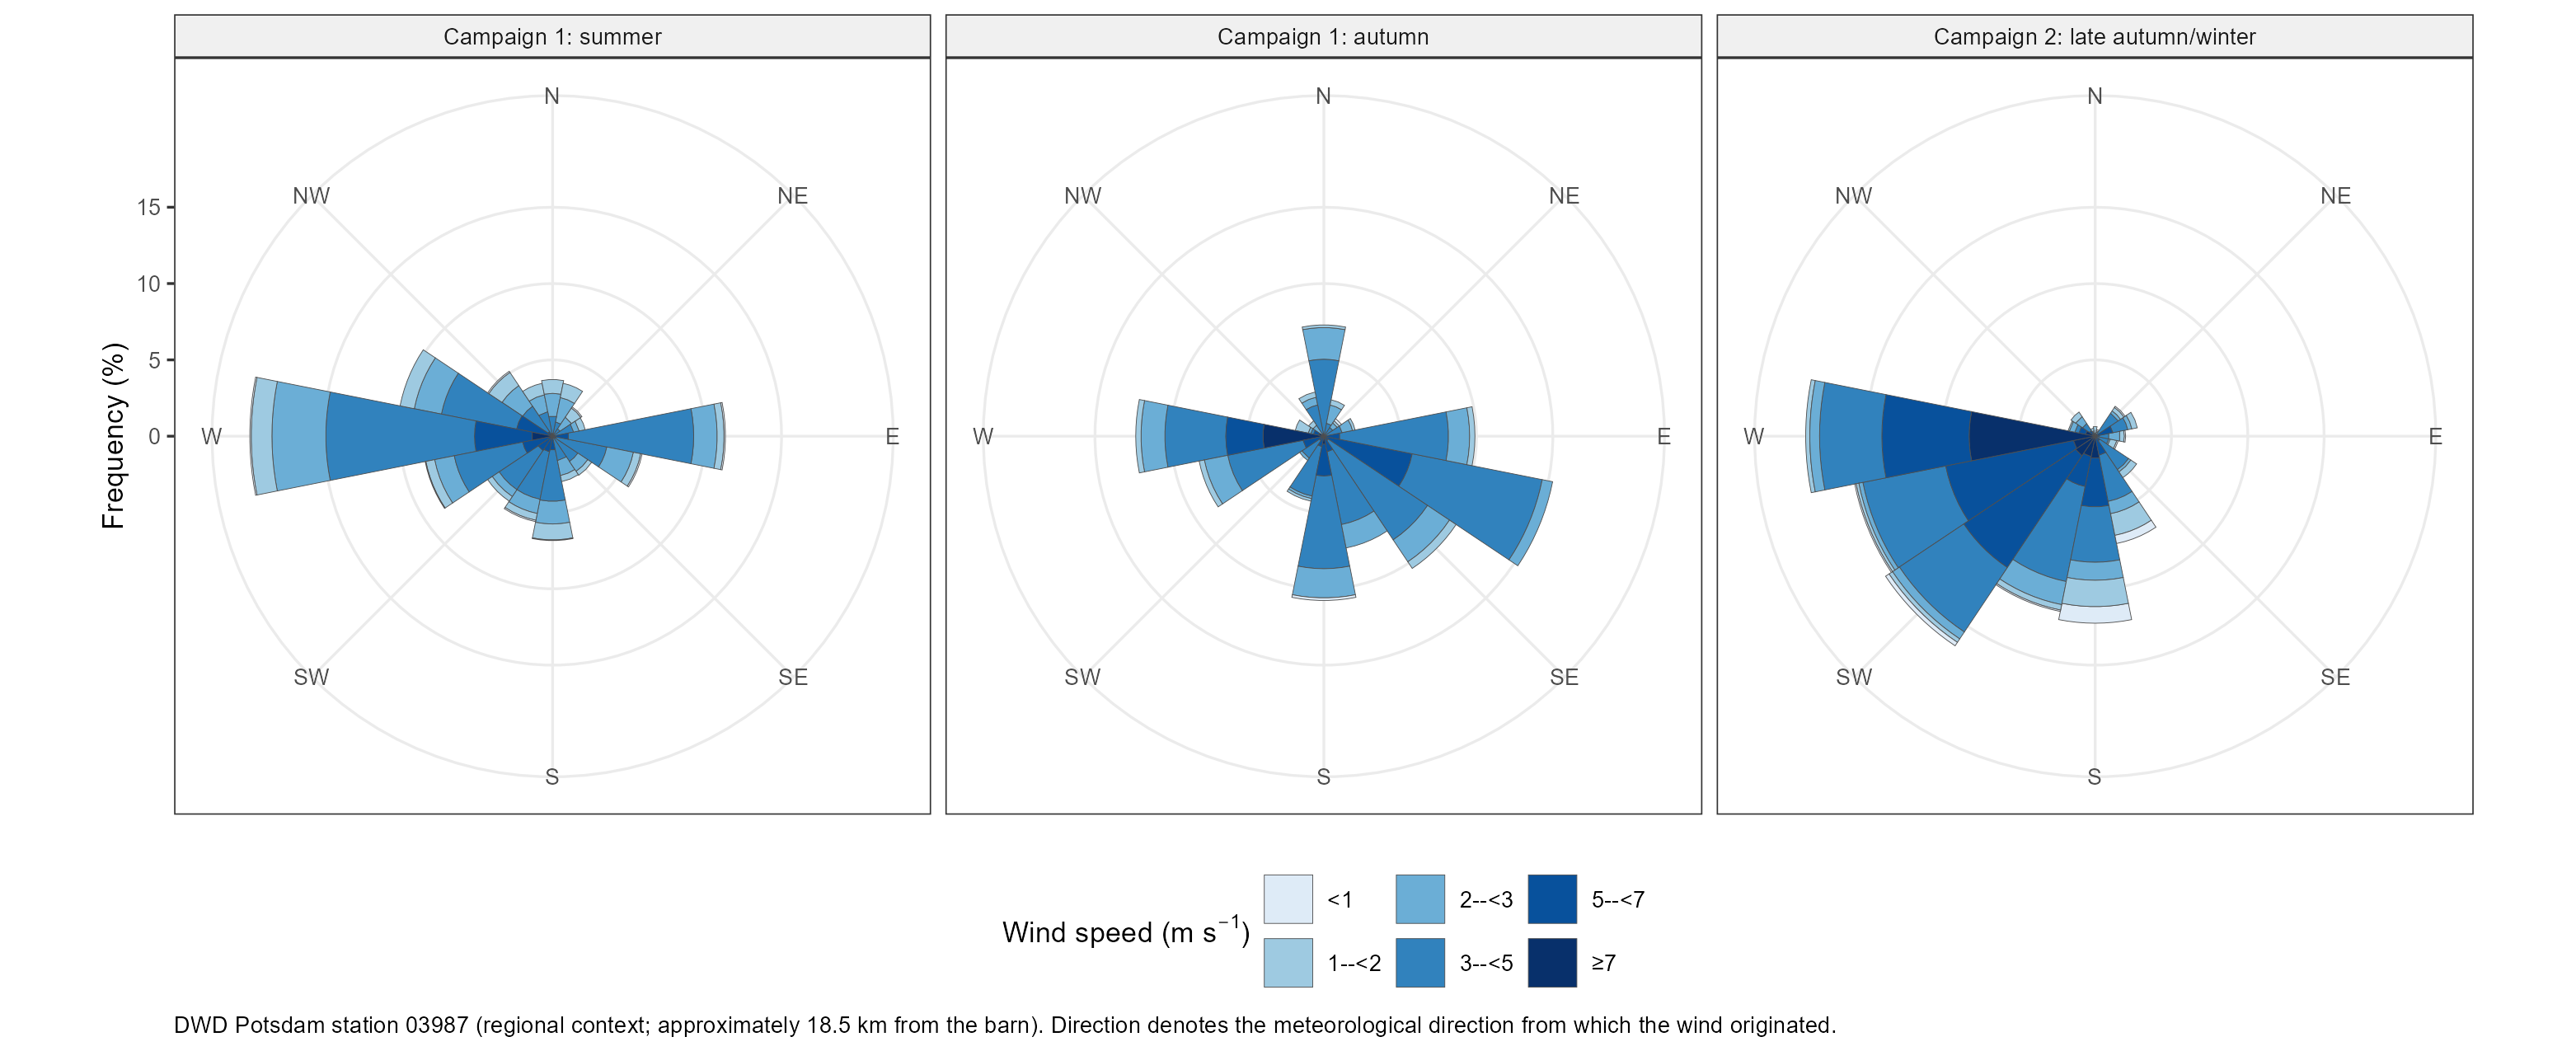
\includegraphics[width=\linewidth]{Fig_DWD_seasonal_wind_roses.png}\caption{Wind direction and speed.}\end{subfigure}
\begin{subfigure}[t]{0.98\textwidth}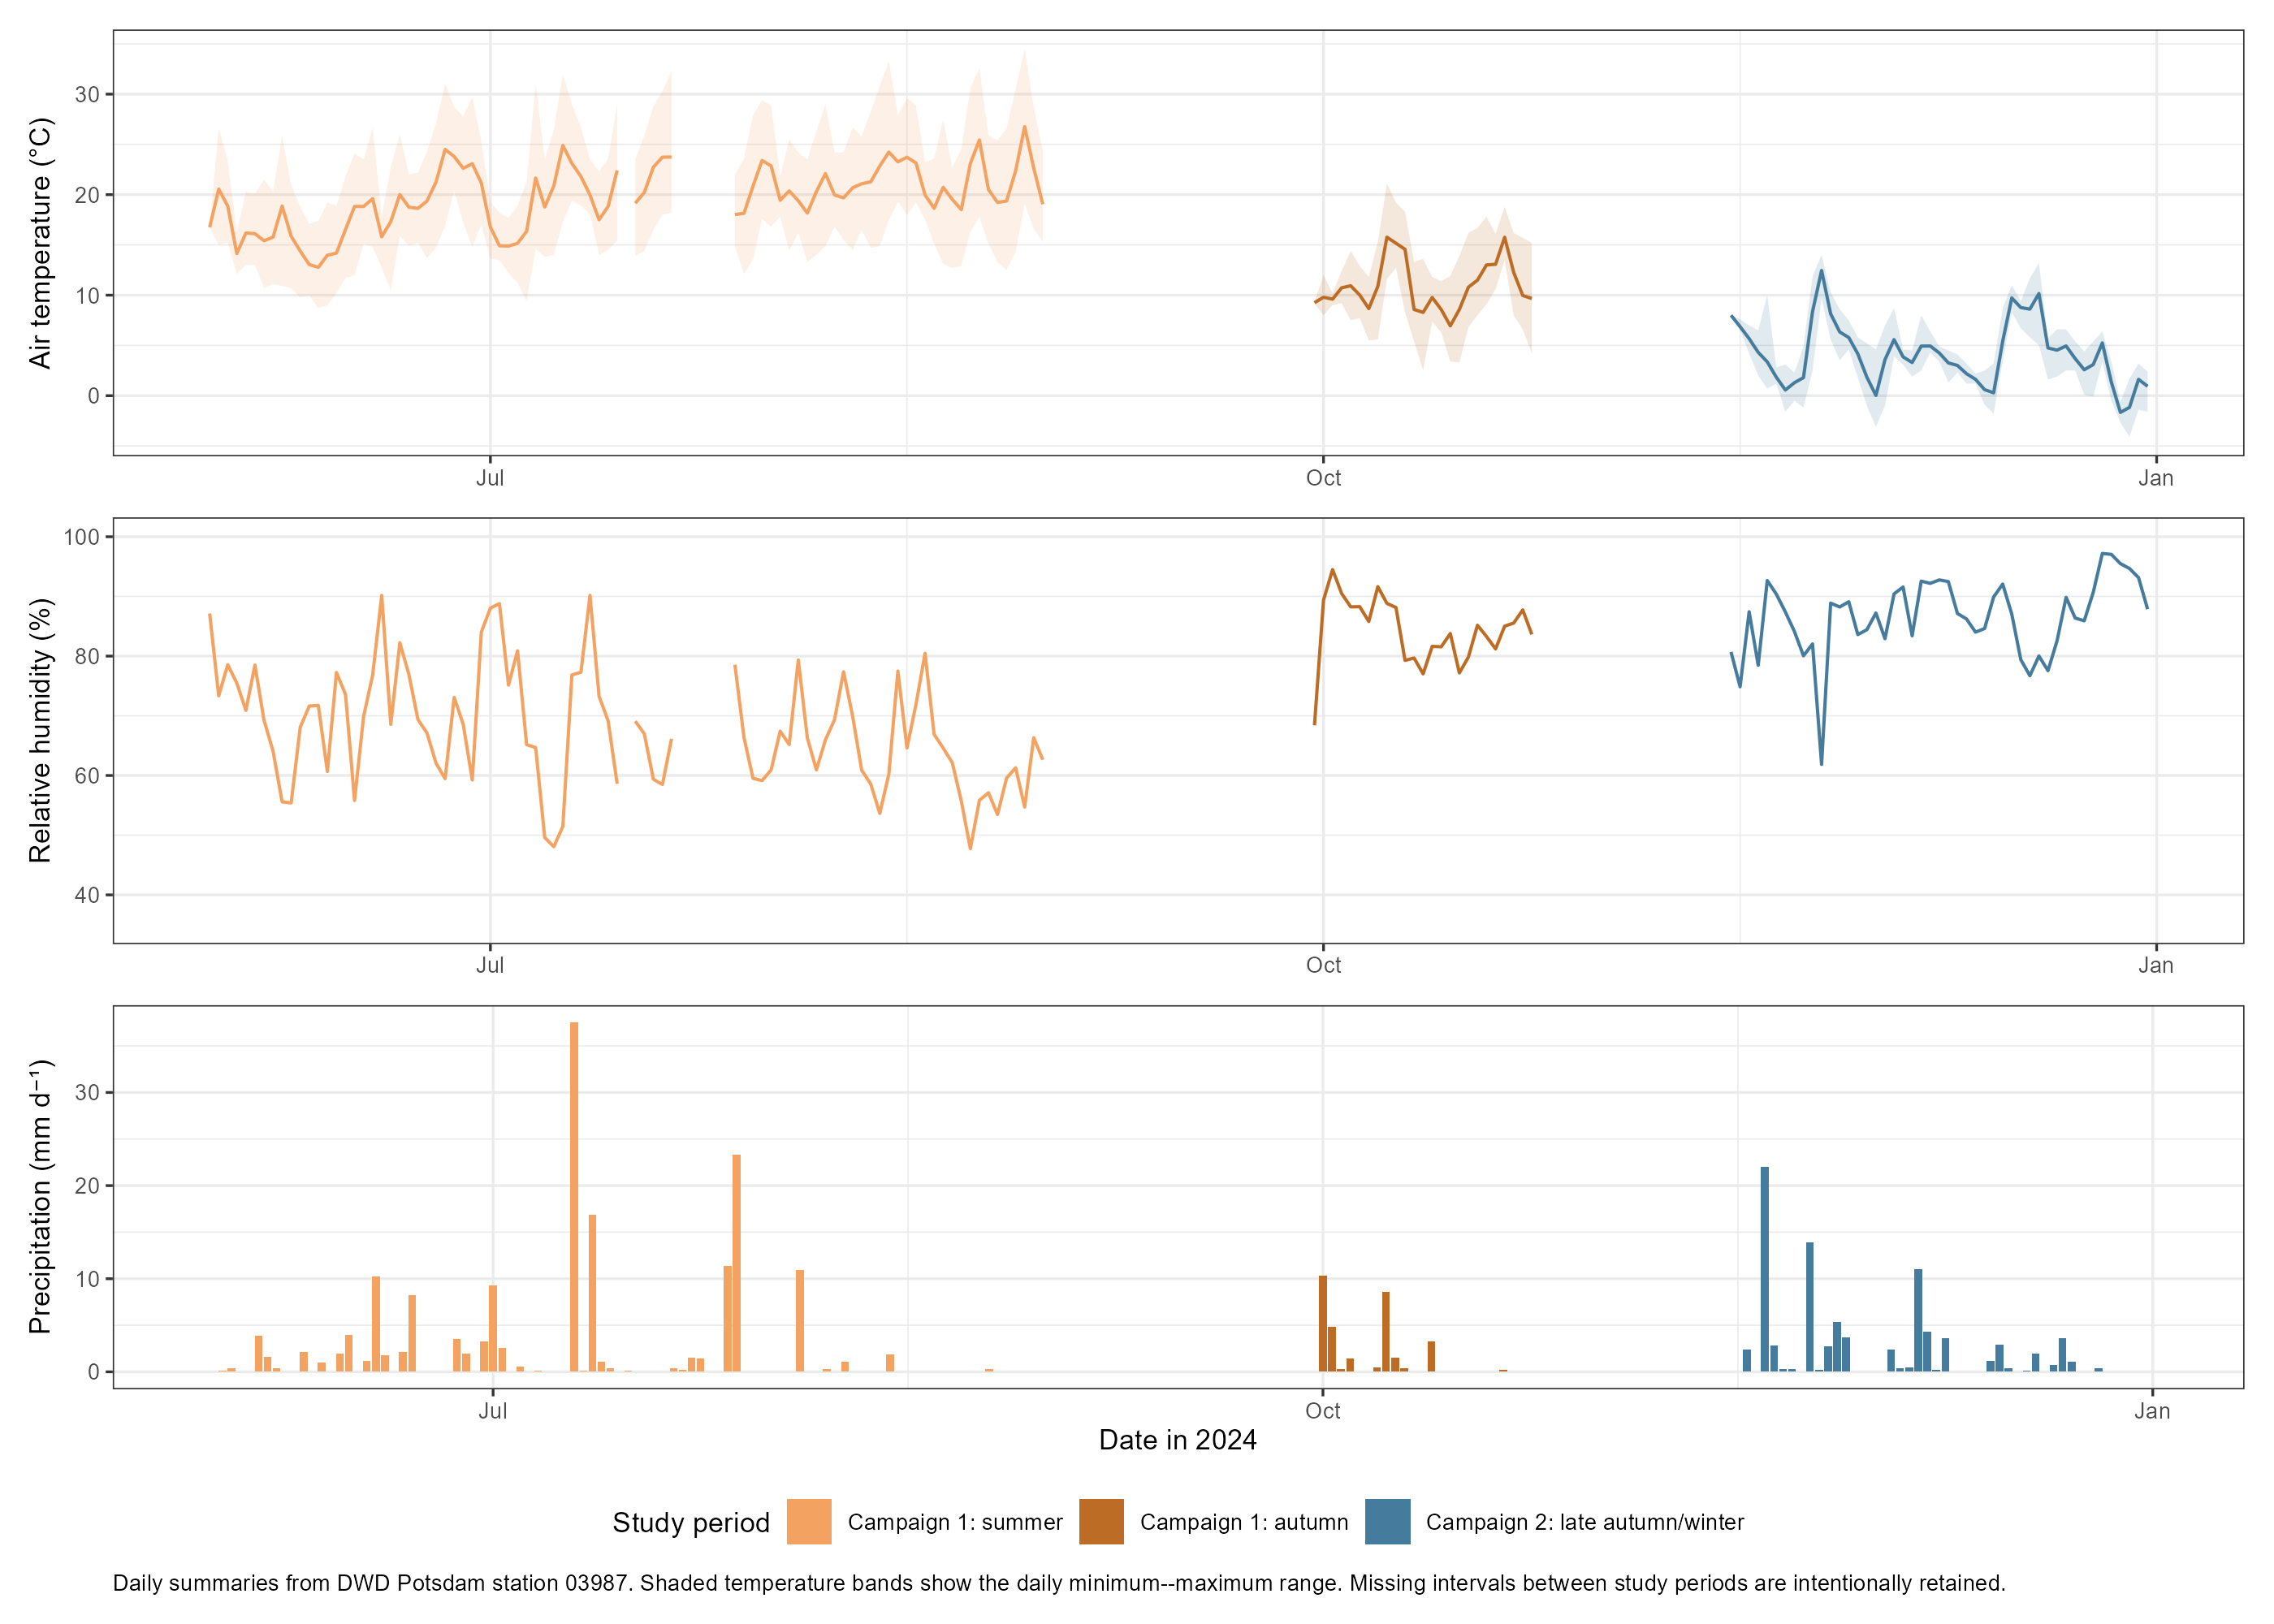
\includegraphics[width=\linewidth]{Fig_DWD_temperature_humidity_precipitation.png}\caption{Temperature, relative humidity and precipitation.}\end{subfigure}
\caption{Meteorological context from the German Meteorological Service. These regional measurements describe seasonal forcing and were not treated as direct measurements of airflow through the barn.}
\label{fig:weather}
\end{figure}

\section{Discussion}
\subsection{Precision is a property of gas, space and time}
The first hypothesis was strongly supported. A statement such as ``the concentration was spatially variable'' is incomplete unless gas and aggregation interval are specified. \(\mathrm{CO_2}\) had the lowest hourly CV, consistent with a broadly distributed animal source and a relatively large ambient baseline. \(\mathrm{NH_3}\) and \(\mathrm{CH_4}\) retained greater spatial variability, consistent with local manure, animal and activity sources. Aggregation reduced much of the transient variability but did not eliminate gas-specific differences. This explains how campaign means may appear stable while hourly sensor placement remains consequential for emission calculations.

The result complements the direct emission analysis of \citet{Janke2020}: their large error at one constant height arose from jointly unresolved concentration and velocity profiles, whereas the present work isolates the concentration component in an occupied barn. The decrease in CV with aggregation should therefore not be interpreted as proof that a temporally averaged single concentration is flux-representative. Concentration and velocity must ultimately be sampled at matching spatial and temporal resolutions.

\subsection{The vertical-increase hypothesis was conditional}
The near-roof increase reported by \citet{Sahu2023} was reproduced most clearly in autumn, but only weakly in summer and not at every horizontal position. This partial support is scientifically more informative than a universal confirmation. It agrees with the gas-specific profiles of \citet{Durso2024} and with the simulation result of \citet{Doumbia2021} that an approximately \SI{3}{m} line represents only some flow regimes. Roof geometry, buoyant animal plumes, fan operation, wind-driven short-circuiting and local sources can each alter the vertical ordering.

The middle SPs at \SI{3.6}{m} were close to the common measurement height and only \SI{1}{m} above the bottom SPs. The dense design was valuable because it bracketed that conventional region with a bottom layer at \SI{2.6}{m} and an uncommon near-roof layer. In summer, the limited middle--bottom separation and small overall gradients made the middle layer comparatively redundant. Its removal in Campaign~2 was therefore a pragmatic outcome of measured heterogeneity. It should not be generalised to barns with different roof slopes, opening geometry, manure management or mechanical air mixing.

Ratio gradients reinforce this interpretation. If vertical differences reflected only uniform dilution, the three ratios would have been stable. Their significant height-by-period interactions instead indicate differing source distributions, chemical behaviour or transport histories. \(\mathrm{NH_3}\) is particularly sensitive to temperature, manure surface conditions and deposition, whereas \(\mathrm{CH_4}\) and \(\mathrm{CO_2}\) arise from overlapping but non-identical animal and manure processes. The ratios are therefore diagnostic, not substitutes for tracer-based ventilation or mass-balance analysis.

\subsection{Wind, neighbouring sources and sensor placement}
Westerly periods did not produce a general concentration rise in these data. Their lower internal means suggest that ventilation enhancement dominated during the observed hours, although this inference remains provisional. A neighbouring naturally ventilated dairy barn could contribute intermittent plumes when upwind, but regional meteorology and internal concentration alone cannot identify that source. A future study should measure approach flow and gas concentrations between the two barns and explicitly test how inter-barn distance, atmospheric stability and plume meandering affect inlet concentrations.

The empirical entropy maps showed that information content was response-specific. This is compatible with the central idea of \citet{Chen2026}, namely that sensor utility depends on the ventilation scenario, but the two entropy quantities are not interchangeable. Chen's method uses CFD-informed fields and an optimisation objective; the present discretised entropy describes observed concentration occupancy under sequential sampling. A defensible sensor network should combine empirical concentration heterogeneity with concurrent velocity sensing, then test candidate configurations by CFD or wind-tunnel simulation.

\subsection{Limitations and future work}
Sequential sampling trades spatial coverage against simultaneity. Although two-hour complete blocks and mixed models reduced this confounding, rapidly changing flow can evolve within a switching cycle. Campaign and season were also partly aliased with network reduction and analyser deployment. DWD measurements were not co-located at the openings. Finally, retaining every positive concentration avoids an arbitrary physical threshold but makes ratio moments sensitive to small denominators; robust block-level summaries are therefore essential.

Future measurements should deploy three-component velocity sensors at spatial and temporal resolutions matched to the gas measurements, especially at vertical openings and near the roof. The measured concentration fields can then constrain CFD simulations or wind-tunnel experiments that resolve inflow, outflow and recirculation. Such work would permit emission-weighted optimisation rather than concentration-only optimisation, and would test whether the reduced network remains valid across barns, seasons and neighbouring-source configurations.

\section{Conclusions}
The apparent precision of barn gas concentration measurements depended jointly on gas, spatial coverage and temporal aggregation. Hourly spatial CV was consistently lowest for \(\mathrm{CO_2}\) and substantially greater for \(\mathrm{CH_4}\) and \(\mathrm{NH_3}\); averaging reduced but did not remove this distinction. Concentrations generally increased from bottom to top in autumn and winter, but the ordering was weaker and spatially inconsistent in summer. Accordingly, H1 was supported, whereas H2 was only conditionally supported.

The middle layer at \SI{3.6}{m} added limited separation during the dense summer observations because it lay only \SI{1}{m} above the bottom layer. Its omission in Campaign~2 was justified as a design consequence of the observed structure, not as evidence for homogeneous mixing. Ratios and entropy maps further demonstrated gas-specific spatial behaviour. For emission applications, concentration sampling should be paired with velocity measurements at matching resolution; until then, reduced networks should be regarded as concentration-representative within the tested barn and periods, not automatically flux-representative.

\section*{Acknowledgements}
The authors thank the staff of the experimental dairy facility for operational support.

\section*{Data and code availability}
The reproducible R workflow used for the reported analysis is version controlled with the manuscript. Raw instrument data are retained by the authors and can be made available subject to institutional data-management requirements.

\bibliographystyle{elsarticle-harv}
\bibliography{references}
\end{document}
